\section{Introduction}
    \subsection{What is Machine Learning}
    
    \begin{enumerate}
        \item Machine Learning 
            \begin{itemize}
                \item Grew out of work in Artificial Intelligence (AI)
                \item New capabilities for computers
            \end{itemize}
        \item Examples: 
            \begin{itemize}
                \item database mining
                \item applications can't programby hand (handwriting recognition, Natural Language Processing (NLP), Computer Vision) 
                \item Neuromorphic applications
            \end{itemize}
           
        \item Definition
            \begin{itemize}
                \item Arthur Samuel(1959) \\
                    \begin{quote}
                        Machine Learning: Field of study that gives computers the ability to learn without being explicitly programmed.

                    \end{quote}
                \item Tom Mitchell(1998) \\
                    \begin{quote}
                         Well-posed Learning Problem: A computer program is said to learn from experience E with respect to some task T and some performance measure P, if its performance on T, as measured by P, improves with experience E. 

                    \end{quote}
           \end{itemize}
        \item Machine Learning in this course:
            \begin{enumerate}
                \item Suupervised Learning
                \item Unsupervised Learning
                \item Others: reinforcement learning, recommender systems
                \item Practical application techniques
            \end{enumerate}
    \end{enumerate}

    
    \subsection{Supervised Learning}

        In supervised learning, the \emph{the right answer} is given. For example:
        \begin{enumerate}
            \item Regression: predict real-valued output.
            \item Classification: predict discrete-valued output.
        \end{enumerate}

    \begin{figure}[h]
        \centering
        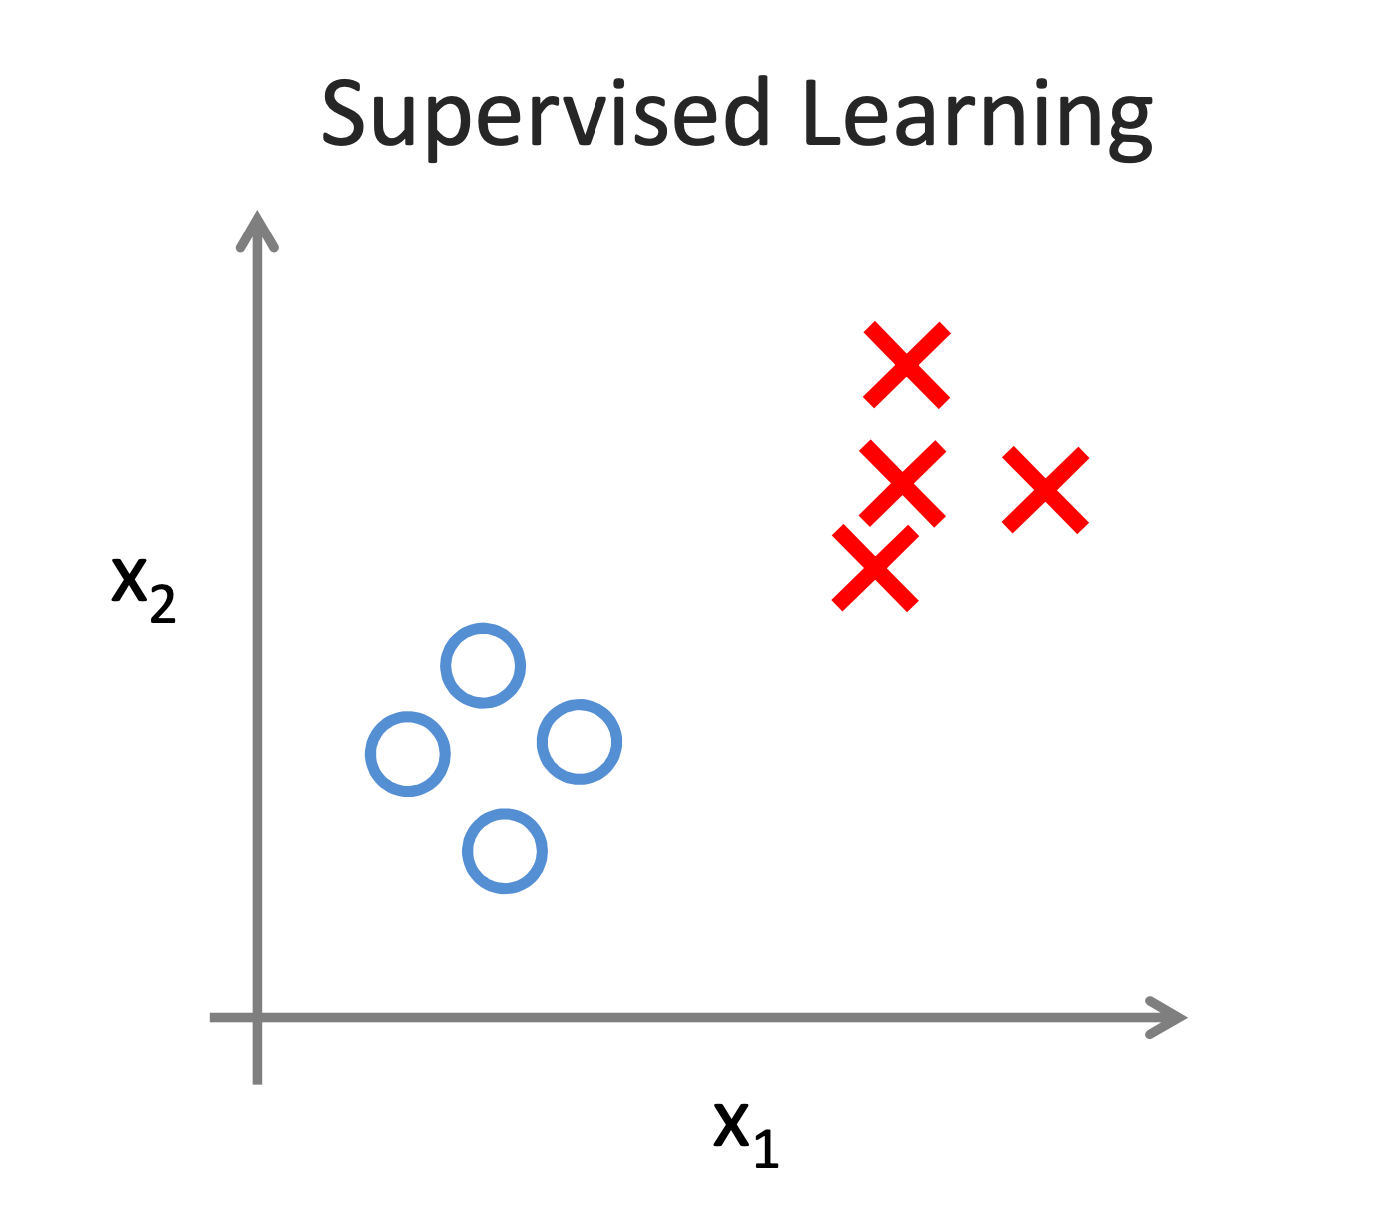
\includegraphics[width=0.5\textwidth]{image/supervised-learning.png}
        \caption{Supervised Learning}
        \label{fig:supervised-learning}
    \end{figure}

    \subsection{Unsupervised Learning}
    The right answer is not given, e.g. cocktail problem (distinguishing two voices from an audio file.)

    \begin{figure}[h]
        \centering
        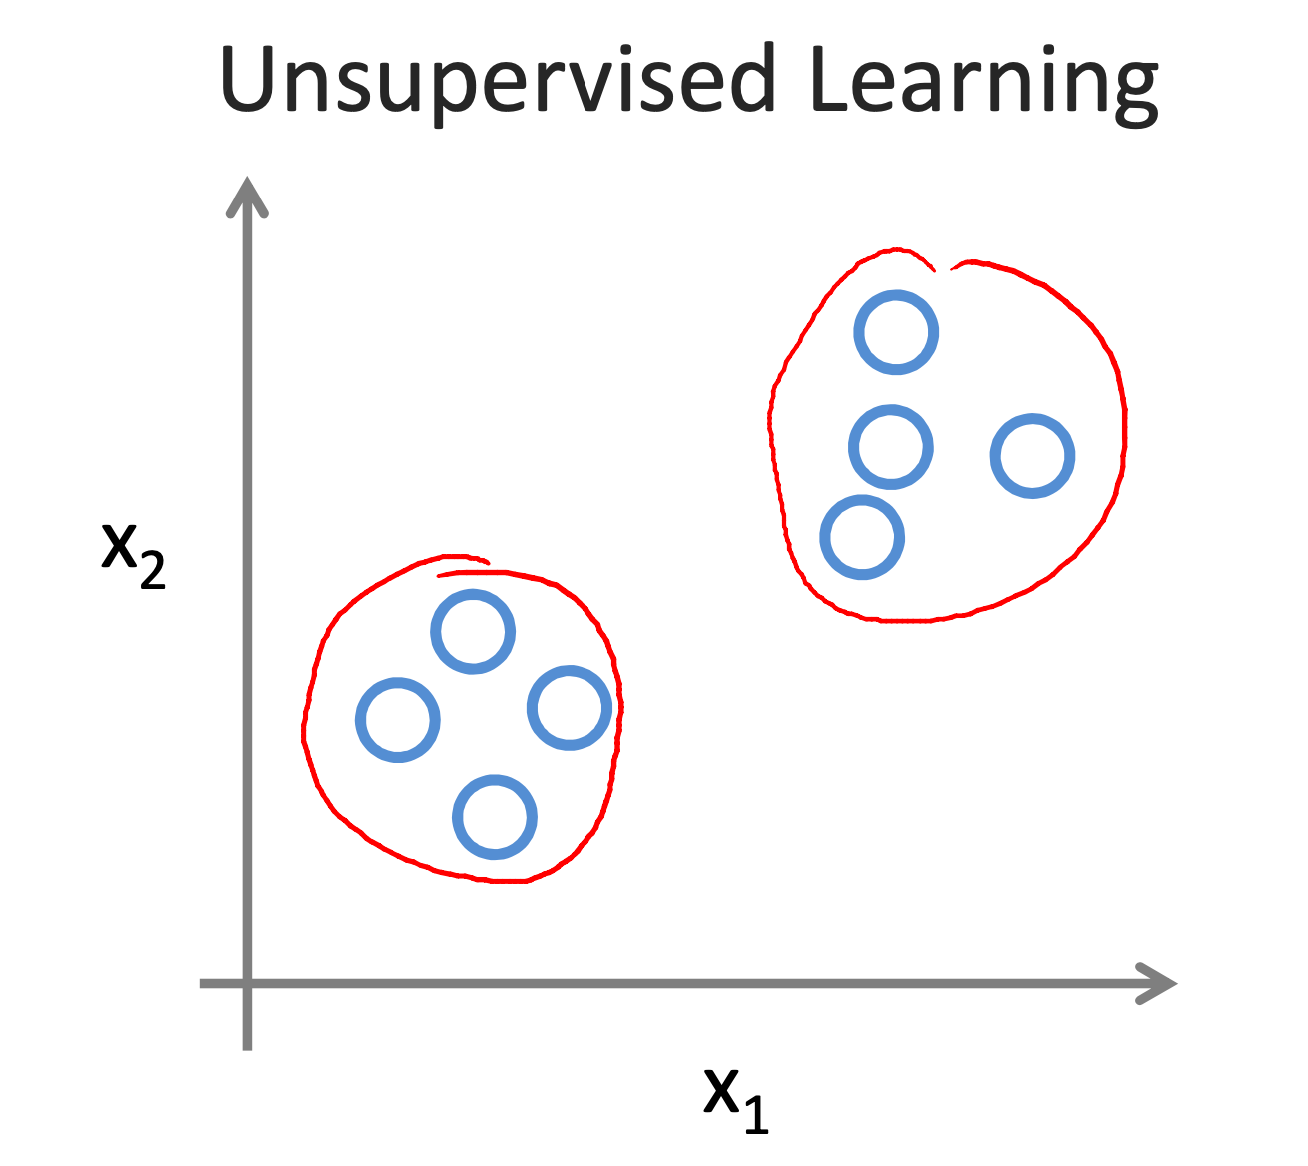
\includegraphics[width=0.5\textwidth]{image/unsupervised-learning.png}
        \caption{Unsupervised learning}
        \label{fig:unsupervised-learning}
    \end{figure}

